\documentclass[aps,pra,twocolumn,reprint,floatfix,amsmath,amssymb]{revtex4-2}

\usepackage{graphicx}
\usepackage{booktabs}
\usepackage{siunitx}
\usepackage[colorlinks=true,linkcolor=blue,citecolor=blue,urlcolor=blue]{hyperref}
\usepackage{xcolor}
\usepackage{braket}

\begin{document}

\title{Single-Pulse Versus Explicit Echoed Multitone SQR for Arbitrary Fock-Conditional Qubit Rotations}
\author{GitHub Copilot}
\affiliation{Quantum Circuits Group}
\date{\today}

\begin{abstract}
The original version of this study tested only one control family: a single standard Gaussian multitone selective-qubit-rotation (SQR) pulse optimized against strict block-diagonal targets in dispersive circuit QED. It did \emph{not} test any echoed, composite, or refocused SQR sequence. That distinction matters, because a poor single-pulse result does not by itself justify a broader impossibility claim about conditional control. This report extends the baseline study by implementing the explicit time-ordered echoed schedule half SQR \(\rightarrow\) \(X_\pi\) \(\rightarrow\) half SQR \(\rightarrow\) \(X_\pi\), with finite Gaussian \(X_\pi\) pulses of duration \SI{40}{ns} about the qubit \(x\) axis, under two fair timing conventions: fixed total duration and fixed active-SQR duration. The physical model keeps only dispersive shifts \(\chi\) and \(\chi'\) and sets cavity Kerr to zero, so the study isolates whether echoed refocusing mitigates the coherent block mismatch seen previously for the single Gaussian multitone ansatz.

The single-pulse baseline remains the best branch overall. Across the echoed-comparison subset, the mean average gate fidelities are \(0.3504\) for the single pulse, \(0.2248\) for the fixed-active echo, and \(0.2190\) for the fixed-total echo. On the strongest structured family-C targets, the echoed sequence is dramatically worse: the family-C median fidelity drops from \(0.7768\) for the single pulse to \(0.2109\) and \(0.1718\) for the fixed-total and fixed-active echoed branches, respectively. On the random family-D ensemble, the echoed sequence is not uniformly harmful: the fixed-active branch improves fidelity in \(38/72\) matched cases and reduces residual blockwise \(Z\) error in \(38/72\), with median deltas \(+0.0027\) in fidelity and \(-0.040\) rad in residual \(Z\). The strongest echoed case reaches fidelity \(0.6061\), improving its matched single-pulse baseline by \(+0.4286\), but it still remains well below the best single-pulse structured result of \(0.8736\).

The revised conclusion is therefore narrower and more precise than the original report: the previous negative result should be read as a failure of the \emph{single-pulse Gaussian multitone SQR ansatz}, not as a general impossibility theorem. The explicit repeated-half echoed construction provides only partial, target-dependent mitigation. It sometimes reduces residual blockwise \(Z\) error for random targets, but it does not rescue the strongest structured cases and does not overturn the broader arbitrary-control failure of the tested ansatz family.
\end{abstract}

\maketitle

\section{Introduction}
Photon-number-selective qubit control is a central primitive in bosonic circuit-QED control, underpinning SNAP, SQR, and hybrid oscillator-qubit gate sets \cite{blais2021cqed,krastanov2015universal,heeres2015snap,heeres2017logical,eickbusch2022fast}. In the ideal dispersive picture, the qubit transition frequency depends on cavity photon number, so the two-dimensional manifolds \(\{\ket{g,n},\ket{e,n}\}\) appear independently addressable. That intuition motivates the hope that a multitone qubit drive can synthesize an arbitrary block-diagonal conditional unitary,
\[
U_{\mathrm{target}} = \sum_{n=0}^{N_{\mathrm{active}}-1} R_n \otimes \ket{n}\bra{n},
\qquad R_n \in SU(2).
\]

The original version of this study asked whether one standard Gaussian multitone SQR pulse, with one tone per active Fock manifold and only per-tone amplitude, phase, and frequency corrections, could realize such arbitrary block control under strict active-subspace metrics. Its answer was negative, but only for that single-pulse ansatz. It did not test any echoed or composite construction. Since echoed refocusing is a standard way to suppress coherent phase accumulation \cite{hahn1950echo}, that omission matters: a poor single-pulse result does not imply that an explicit echoed SQR sequence must fail for the same reason.

This extension addresses that gap directly. We preserve the validated single-pulse baseline, then add the explicit user-requested time-ordered sequence
\[
\text{half SQR} \rightarrow X_\pi \rightarrow \text{half SQR} \rightarrow X_\pi,
\]
implemented with finite Gaussian \(X_\pi\) pulses and identical first and second half-SQR waveforms. The central questions are: Did the original report test only the single pulse? Does the explicit echoed sequence improve arbitrary conditional rotations? If improvement occurs, is it mainly due to cancellation of unwanted block-dependent \(Z\) phase? The remainder of the paper answers those questions quantitatively. Section~II defines the model, waveform parameterizations, and metrics. Section~III reports the single-versus-echo comparison. Section~IV validates the extension. Sections~V and~VI interpret the result and state the practical conclusion.

\section{System and Methods}

\subsection{Hamiltonian and basis convention}
We model a dispersively coupled qubit-cavity system with Fock-conditioned qubit frequency
\[
\omega_q^{(n)} = \omega_q + \chi n + \chi' n(n-1),
\]
and lab-frame Hamiltonian
\begin{align}
\frac{H(t)}{\hbar} &= \omega_c a^\dagger a + \frac{\omega_q}{2}\sigma_z
+ \left[\chi a^\dagger a + \chi' a^\dagger a(a^\dagger a - 1)\right]\frac{I+\sigma_z}{2} \\
&\quad + \frac{1}{2}\left[\Omega(t)\sigma_+ + \Omega^*(t)\sigma_-\right].
\end{align}
Here \(a\) is the cavity annihilation operator, \(\sigma_\pm\) are qubit ladder operators, and the cavity self-Kerr is set to zero throughout the main study. Simulations use \texttt{cqed\_sim} in the rotating frame defined by the bare qubit and cavity frequencies, so the active manifolds differ only through the dispersive shifts.

Throughout the study we follow the qubit-first \texttt{cqed\_sim} convention: logical operators are restricted in the ordered basis
\[
(\ket{g,0},\ket{e,0},\ket{g,1},\ket{e,1},\ldots).
\]
The global active-subspace dimension is therefore \(d = 2N_{\mathrm{active}}\).

\subsection{Single-pulse and echoed waveform parameterizations}
The baseline control family is the standard Gaussian multitone SQR ansatz,
\[
\Omega_{\mathrm{single}}(t) = g_T(t)\sum_{n=0}^{N_{\mathrm{active}}-1} A_n e^{-i[(\omega_n^{(0)} + d\omega_n)t + (\phi_n^{(0)} + d\alpha_n)]},
\qquad 0 \le t \le T,
\]
with Gaussian envelope
\[
g_T(t) = \exp\!\left[-\frac{(t-T/2)^2}{2(\sigma_T T)^2}\right],
\qquad \sigma_T = \frac{1}{6}.
\]
The optimizer varies \((d\lambda_n,d\alpha_n,d\omega_n)\) per tone; the effective tone amplitude is absorbed into \(A_n\), and the carrier frequencies \(\omega_n^{(0)}\) are the manifold transition frequencies supplied to the conditioned-multitone builder.

The echoed extension keeps the same half-SQR waveform in both halves and inserts finite Gaussian qubit \(\pi\) pulses,
\[
X_\pi = -i\sigma_x,
\qquad
\Omega_\pi(t) = A_\pi g_\pi(t)e^{-i\omega_{n=0}t},
\]
with duration \(\tau_\pi = \SI{40}{ns}\), phase \(0\), manifold-0 carrier, and Gaussian shape parameter \(\sigma_\pi = 0.25\). Under the study's right-action convention, the time-ordered pulse schedule half-SQR then \(X_\pi\) then half-SQR then \(X_\pi\) corresponds blockwise to
\[
U_{\mathrm{echo}}^{(n)} = X_\pi W_n X_\pi W_n.
\]
The ideal repeated-half design uses
\[
W_n = X_\pi^\dagger R_n^{1/2},
\]
so that \(U_{\mathrm{echo}}^{(n)} = R_n\) in the ideal manifold-resolved picture. Two fair timing conventions are tested:
\begin{align}
T_h^{\mathrm{fixed\ total}} &= \frac{T-2\tau_\pi}{2}, \\
T_h^{\mathrm{fixed\ active}} &= \frac{T}{2},
\end{align}
where \(T\) is the single-pulse baseline duration. The first holds the total gate time fixed, while the second holds the total active SQR time fixed and adds the two \(X_\pi\) pulses on top.

\subsection{Study design, objective, and diagnostics}
The preserved baseline study contains 192 optimized single-pulse cases over four target families A--D, \(N_{\mathrm{active}} = 2,3,4,5\), \(|\chi|T/2\pi\in\{1,3,5,7\}\), and both \(\chi\)-only and \(\chi+\chi'\) models. The echoed extension focuses on the most informative subset: family C, which was the strongest structured family in the original report, and family D, the Haar-random ensemble that most directly tests arbitrary control. For the echoed extension we sweep \(N_{\mathrm{active}}=2,3,4\), \(|\chi|T/2\pi\in\{1,3,5\}\), both model variants, and the same four family-D seeds per operating point as the baseline subset, yielding 90 baseline rows and 180 echoed rows.

Optimization is performed against the strict active-subspace target operator. The primary fidelity metrics are
\[
\mathcal{F}_{\mathrm{pro}} = \frac{\left|\mathrm{Tr}\left(U_{\mathrm{target}}^\dagger U_{\mathrm{res}}\right)\right|^2}{d^2},
\qquad
\mathcal{F}_{\mathrm{avg}} = \frac{d\,\mathcal{F}_{\mathrm{pro}} + 1}{d+1},
\]
with \(d=2N_{\mathrm{active}}\) for the full restricted operator and \(d=2\) for each Fock block. For per-block coherent-error analysis we form the block error unitary
\[
E_n = R_n^\dagger \widetilde{R}_n = \exp\!\left[-\frac{i}{2}(\delta\theta_{n,x}\sigma_x + \delta\theta_{n,y}\sigma_y + \delta\theta_{n,z}\sigma_z)\right].
\]
We then report the residual blockwise \(Z\) error \(|\delta\theta_{n,z}|\) and the transverse coherent error
\[
\delta\theta_{n,\perp} = \sqrt{\delta\theta_{n,x}^2 + \delta\theta_{n,y}^2},
\]
along with worst-block fidelity, Frobenius error, state-transfer diagnostics, and superposition-state validation.

\begin{table*}[t]
  \centering
  \caption{Fixed physical and numerical parameters for the echoed comparison.}
  \begin{tabular}{@{}lll@{}}
    \toprule
    Parameter & Value & Unit \\
    \midrule
$\omega_q/2\pi$ & 6.150 & GHz \\
    $\omega_c/2\pi$ & 5.241 & GHz \\
    $\alpha/2\pi$ & -255 & MHz \\
    $\chi/2\pi$ & -2.84 & MHz \\
    $\chi'/2\pi$ & -21 & kHz \\
    $K/2\pi$ & 0 & kHz \\
    $N_{\mathrm{tr}}$ & 2 & levels \\
    $N_{\mathrm{cav}}$ & $N_{\mathrm{active}}+2$ & Fock states \\
    $\Delta t$ & 4 & ns \\
    Single-pulse envelope width & $\sigma_T=1/6$ & fraction of $T$ \\
    Echo \(X_\pi\) duration & 40 & ns \\
    Echo \(X_\pi\) axis / phase & $x$, $0$ & --- \\
    \bottomrule
  \end{tabular}
  \label{tab:params}
\end{table*}

\section{Results}

\subsection{What the previous report did and did not test}
The previous report tested only the single Gaussian multitone SQR pulse. It did not include any echoed, composite, or refocused construction. That scope distinction is now machine-checked by the echoed validation script, which verifies that the earlier validated best branch is \texttt{single\_pulse} and that the newly added explicit sequence order is \texttt{half\_sqr, x\_pi, half\_sqr, x\_pi}. The original negative result should therefore be interpreted narrowly: it established failure of the single-pulse Gaussian ansatz, not a general no-go theorem for all echoed SQR variants.

\subsection{Single pulse remains the best branch overall}
Figure~\ref{fig:branch-means} summarizes the branch-level statistics on the matched comparison subset. The single-pulse branch remains strongest overall: its mean average gate fidelity is \(0.3504\), versus \(0.2248\) for \texttt{echoed\_fixed\_active} and \(0.2190\) for \texttt{echoed\_fixed\_total}. The same ordering holds for mean worst-block fidelity. Echo does not deliver a branch-wide improvement in either fidelity or coherent-error averages.

The best single-pulse case is still the structured family-C target \texttt{chi\_plus\_chiprime\_na2\_chiT1p0\_familyC}, which reaches average gate fidelity \(0.873625\). The best echoed case, \texttt{chi\_only\_na3\_chiT5p0\_familyD\_seed317160} under \texttt{echoed\_fixed\_total}, reaches only \(0.606132\). The best echoed random target therefore improves substantially over its matched single-pulse baseline, but still remains well below the strongest structured single-pulse result.

\begin{figure}[t]
  \centering
  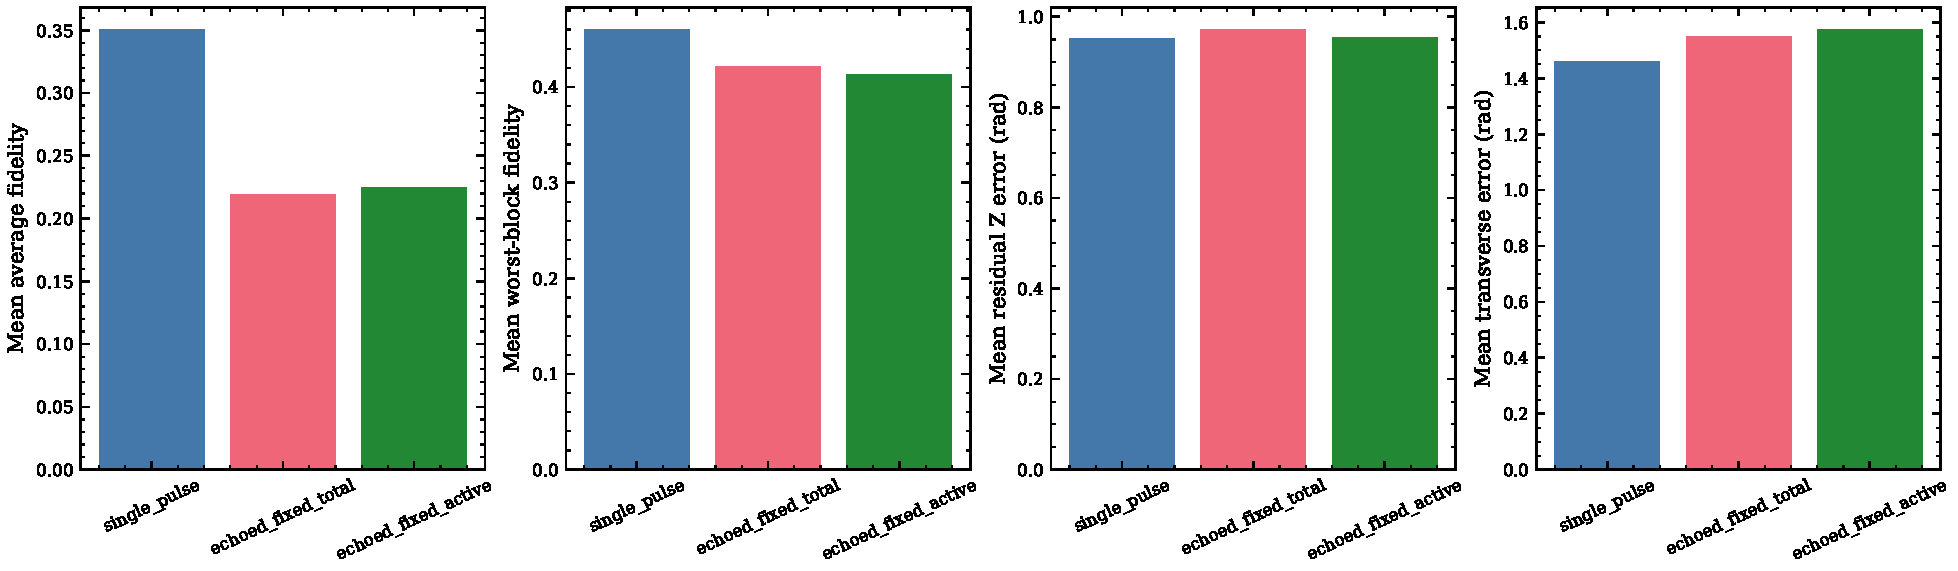
\includegraphics[width=\linewidth]{../figures/echo_branch_metric_means.pdf}
  \caption{Branch-level means on the 90-case comparison subset. The single pulse remains best on average in fidelity and worst-block fidelity, while both echoed branches slightly worsen the mean residual-\(Z\) and transverse coherent-error metrics.}
  \label{fig:branch-means}
\end{figure}

\subsection{The echoed sequence fails badly on structured family C}
Figure~\ref{fig:duration-scan} shows the most decisive qualitative result. For the structured family-C targets, the single pulse has median fidelity \(0.7768\), nearly independent of \(|\chi|T/2\pi\) across the scanned range. Both echoed branches collapse that median to roughly \(0.21\) or lower at every duration. The matched-case medians sharpen the point:
\begin{align*}
\mathrm{median}\,\Delta \mathcal{F}_{\mathrm{avg}} &= -0.560351 \quad \text{(fixed total)}, \\
\mathrm{median}\,\Delta \mathcal{F}_{\mathrm{avg}} &= -0.588711 \quad \text{(fixed active)},
\end{align*}
with improved-fidelity counts of \(0/18\) in both cases. This is not a marginal tradeoff. The explicit repeated-half echo is qualitatively worse than the baseline single pulse on the very structured family that previously looked most promising.

\begin{figure}[t]
  \centering
  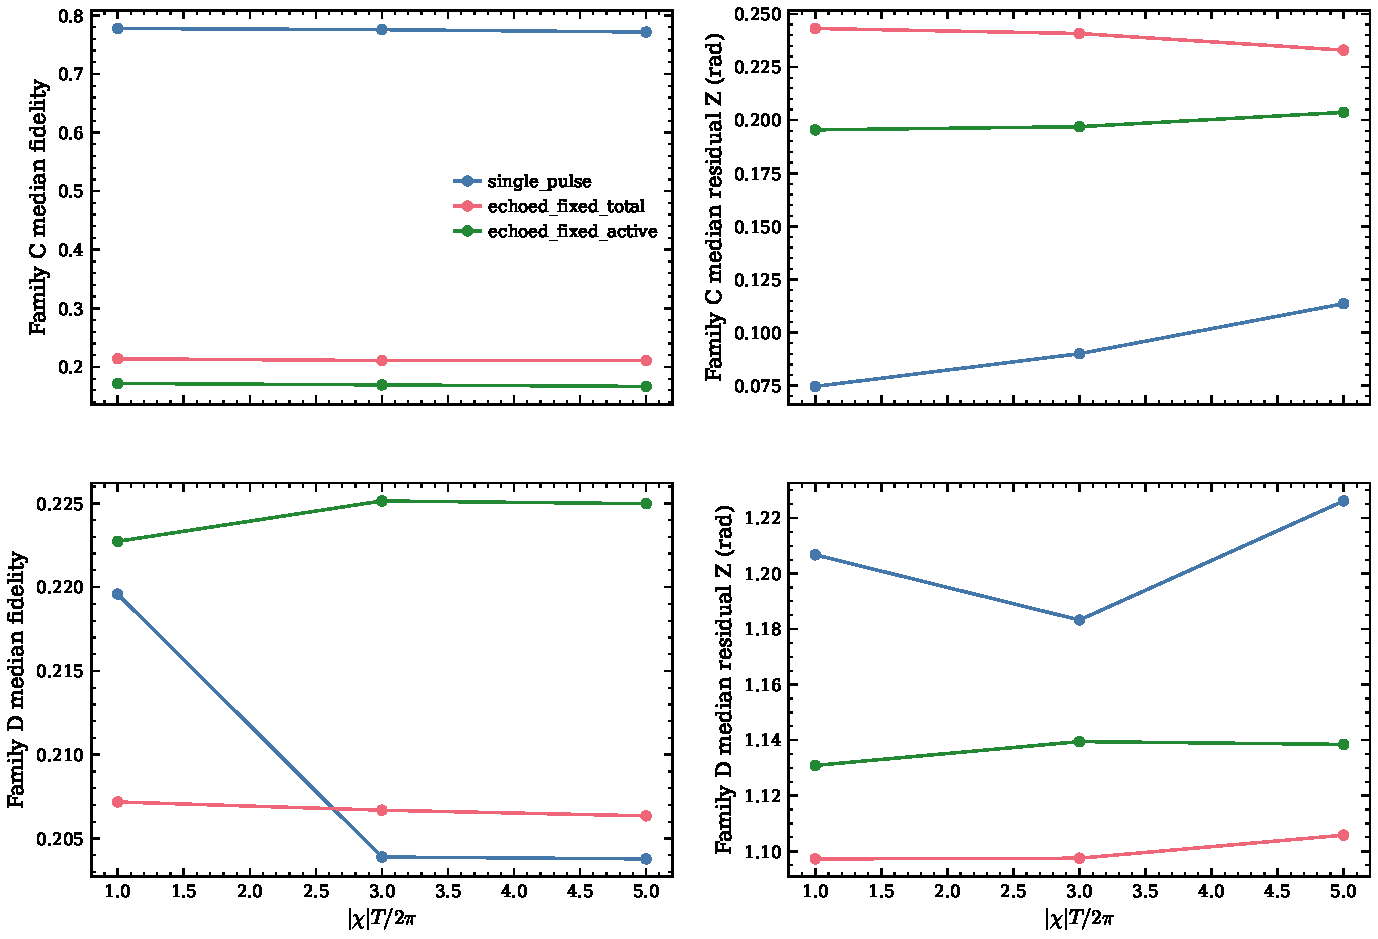
\includegraphics[width=\linewidth]{../figures/echo_duration_scan.pdf}
  \caption{Family-C and family-D median fidelity and residual-\(Z\) error versus \(|\chi|T/2\pi\). Echo severely degrades the structured family-C frontier at every scanned duration, while the family-D behavior is mixed and only weakly favorable for the fixed-active branch.}
  \label{fig:duration-scan}
\end{figure}

\subsection{Random family D shows only partial, target-dependent mitigation}
The family-D ensemble is the stronger test of arbitrary block control. Here the echoed sequence is not uniformly harmful. The fixed-active echoed branch improves fidelity in \(38/72\) matched cases and reduces mean residual-\(Z\) error in \(38/72\), with median deltas
\[
\Delta \mathcal{F}_{\mathrm{avg}} = +0.002700,
\qquad
\Delta \overline{\delta\theta_z} = -0.040052~\mathrm{rad}.
\]
The fixed-total branch is slightly weaker, with median fidelity delta \(-0.002212\) and median residual-\(Z\) delta \(+0.026359\) rad. The strongest random-case fidelity gain is \(+0.428582\), achieved by the same best echoed case that reaches \(0.606132\). The strongest reduction in mean residual-\(Z\) error is \(-0.635356\) rad for \texttt{chi\_only\_na4\_chiT3p0\_familyD\_seed318160} under \texttt{echoed\_fixed\_total}.

Even these positive cases do not amount to a rescue of arbitrary control. The family-D medians remain near \(0.21\) for all three branches, and the best echoed result is still far below the best structured single-pulse case. The echoed construction helps some random targets, but only selectively.

\subsection{Improvement is not explained by residual-\texorpdfstring{$Z$}{Z} cancellation alone}
The user's most specific hypothesis was that the single-pulse obstruction might be largely block-dependent residual-\(Z\) accumulation and that echo would cancel it. The matched echoed-minus-single scatter data do not support such a simple explanation. For family C, the echoed branches generally move to larger residual-\(Z\) error and lower fidelity simultaneously. For family D, some cases do move into the favorable regime of reduced residual-\(Z\) and improved fidelity, but many do not, and transverse coherent error often worsens even when residual \(Z\) improves.

This is the core physical conclusion of the extension. Echo sometimes suppresses one component of the coherent block error, but the remaining transverse mismatch is still large enough to limit the full blockwise unitary. The best echoed case illustrates that behavior directly: its per-block residual-\(Z\) errors are \((0.363, 1.301, 1.026)\) rad, while its transverse coherent errors are \((0.942, 0.235, 1.713)\) rad. The worst block still has average gate fidelity only \(0.5289\).

\section{Validation}

\subsection{Sanity checks}
The original single-pulse study had already passed the sanity checks recorded in \texttt{data/validation\_summary.json}: zero-drive replay is nearly identity in the chosen frame, and a single-manifold target can be reproduced at high fidelity. The echoed extension inherits that baseline validation and adds an explicit sequence-order check. The dedicated echoed validation file \texttt{data/echo\_comparison\_validation.json} records the time ordering
\[
\texttt{half\_sqr, x\_pi, half\_sqr, x\_pi}
\]
as passed.

\subsection{Convergence analysis}
The best echoed case was replayed with a finer compilation step and a larger cavity truncation. Reducing the time step from \SI{4}{ns} to \SI{2}{ns} changes the best echoed fidelity from \(0.6061322135\) to \(0.6053269943\), a shift of only \(-8.05\times10^{-4}\). Increasing the cavity truncation by two levels changes the same fidelity to \(0.6061328393\), a shift of only \(+6.26\times10^{-7}\). These deltas are too small to affect the qualitative verdict.

\subsection{Literature comparison}
Literature comparison is marked not applicable. This is an original optimization-and-analysis study rather than a direct reproduction benchmark. The relevant validation standard is therefore internal consistency, convergence, and artifact-backed reproducibility rather than percent-error agreement with a published figure.

\section{Discussion}
The revised evidence supports three distinct statements.

First, the old report tested only the single Gaussian multitone pulse. Any interpretation of that report as a statement about general echoed or composite SQR was too broad.

Second, the newly tested explicit echoed sequence does not overturn the baseline negative conclusion. On the strongest structured family-C cases it is dramatically worse, not marginally worse. That rules out the simplest optimistic interpretation that the single-pulse problem was merely an uncancelled blockwise phase that an ordinary echoed refocusing pattern would remove.

Third, the echoed extension is not useless. On random family-D targets it sometimes improves fidelity and sometimes reduces residual-\(Z\) error substantially. The strongest echoed gain of \(+0.4286\) shows that the repeated-half sequence can matter nontrivially on some targets. But those wins remain target-dependent and incomplete. The branch means remain below the single-pulse baseline, and the best echoed case is still far from a high-fidelity arbitrary-control demonstration.

The resulting interpretation is therefore more nuanced than the original manuscript. The data support a narrow ansatz-level negative claim: the single-pulse Gaussian multitone family is inadequate for strict arbitrary block control, and the explicit repeated-half echoed extension only partially mitigates that limitation. They do \emph{not} support a universal impossibility theorem about all echoed or segmented conditional-control strategies. Richer composite constructions with independently optimized halves, different refocusing axes, or optimal-control segments remain open possibilities.

\section{Conclusion}
The explicit echoed test changes the wording of the conclusion, but not the practical verdict. The previous report should now be read as showing failure of the single-pulse Gaussian multitone SQR ansatz, not as a general no-go statement. After adding the exact user-requested sequence half SQR \(\rightarrow\) \(X_\pi\) \(\rightarrow\) half SQR \(\rightarrow\) \(X_\pi\), the best branch is still the single pulse. Echo badly degrades the structured family-C cases, while only partially helping a subset of random family-D cases. The evidence therefore points to a deeper coherent-control limitation than uncancelled residual blockwise \(Z\) phase alone. For practical use, the best current conclusion is: single-pulse Gaussian multitone SQR is not sufficient for strict arbitrary block-diagonal control, and the repeated-half echoed extension does not rescue that limitation.

\section{Limitations and Future Work}

\subsection{Known Limitations}
This extension tests exactly one echoed family: identical first and second half-SQR waveforms separated by finite Gaussian \(X_\pi\) pulses. The two halves are not independently optimized, and the second half is not phase shifted or reparameterized. The main optimization still uses a two-level qubit model and omits cavity Kerr, open-system noise, and transmon leakage, so the reported obstruction is a coherent closed-system limitation of the tested ansatz family. Finally, the echoed sweep focuses on families C and D; it does not re-run families A and B because they are less diagnostic for the user's question.

\subsection{Suggested Improvements}
\begin{itemize}
  \item \textbf{[P1 | MEDIUM]} Optimize the two half-SQR waveforms independently rather than forcing an identical repeated-half construction.
  \item \textbf{[P1 | MEDIUM]} Test alternative refocusing pulses and axes, including imperfect-manifold-aware \(X_\pi\) calibrations, to separate echo-design limits from the specific manifold-0 Gaussian \(X_\pi\) used here.
  \item \textbf{[P2 | HIGH]} Compare the Gaussian ansatz family against segmented or GRAPE-style controls \cite{khaneja2005grape} to determine whether the remaining failure is ansatz-limited or more fundamental.
  \item \textbf{[P2 | MEDIUM]} Replay the strongest single and echoed cases with a qutrit transmon model and realistic decoherence to separate coherent block mismatch from leakage and noise sensitivity.
\end{itemize}

\subsection{Open Questions}
Which block-diagonal targets are genuinely helped by echoed refocusing, and what geometric property of those targets predicts improvement? Is the dominant obstruction a shortage of independently tunable blockwise transverse controls, or can a richer composite schedule convert the small residual-\(Z\) gains seen on family D into a broad fidelity improvement?

\bibliographystyle{apsrev4-2}
\bibliography{references}

\appendix

\section{Detailed Results and Data}
The main machine-readable outputs now come in two layers. The preserved single-pulse baseline is stored in \texttt{data/study\_results.json}, \texttt{data/machine\_summary.json}, and \texttt{artifacts/cases/}. The explicit echoed extension is stored in \texttt{data/echo\_comparison\_results.json}, \texttt{data/echo\_comparison\_summary.json}, \texttt{data/echo\_comparison\_results.csv}, and the per-case JSON/NPZ files under \texttt{artifacts/echo\_comparison/}. The summary markdown file \texttt{data/echo\_comparison\_summary.md} provides the human-readable branch and matched-delta tables used in the main text.

\begin{figure}[t]
  \centering
  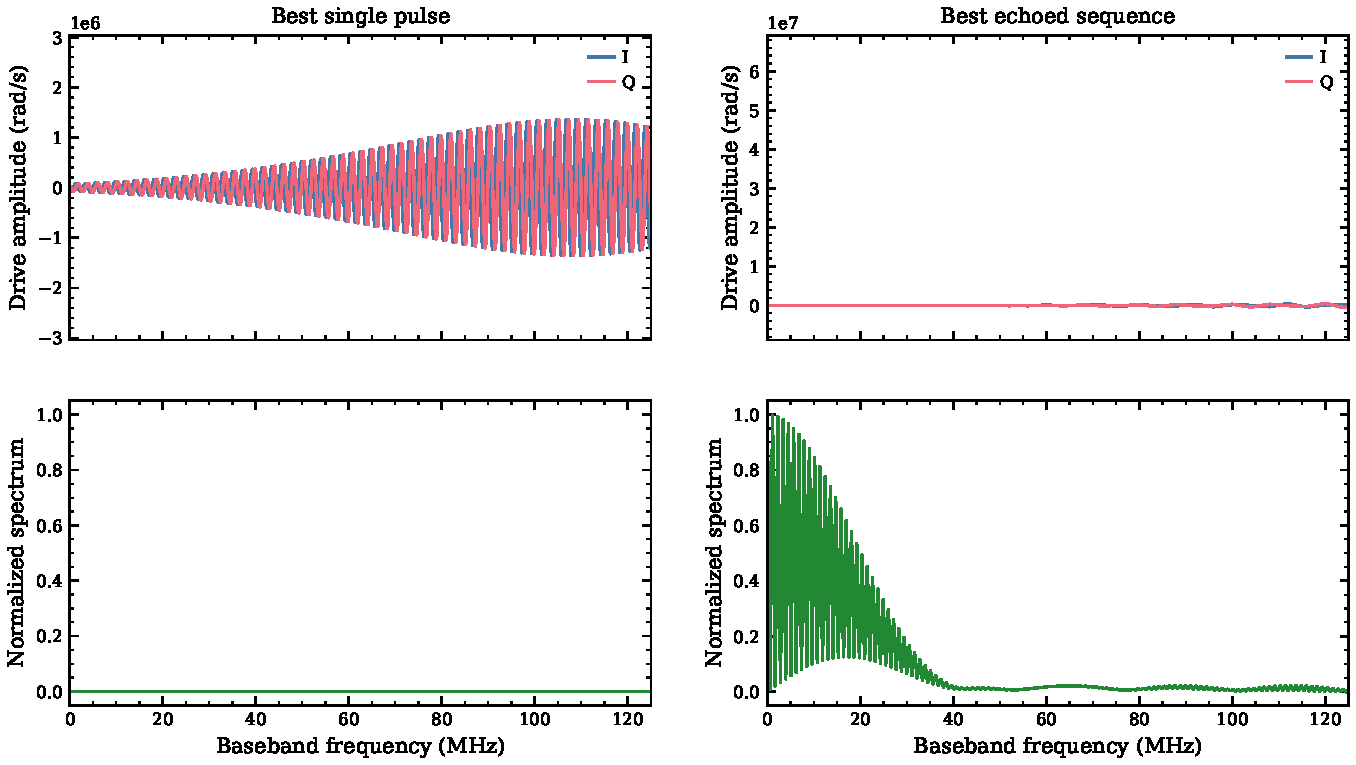
\includegraphics[width=\linewidth]{../figures/echo_best_waveforms.pdf}
  \caption{Time-domain waveforms and frequency-domain spectra for the best single-pulse baseline and the best echoed sequence. The right column corresponds to the best echoed random-target case \texttt{chi\_only\_na3\_chiT5p0\_familyD\_seed317160} under \texttt{echoed\_fixed\_total}.}
  \label{fig:best-waveforms}
\end{figure}

\begin{figure}[t]
  \centering
  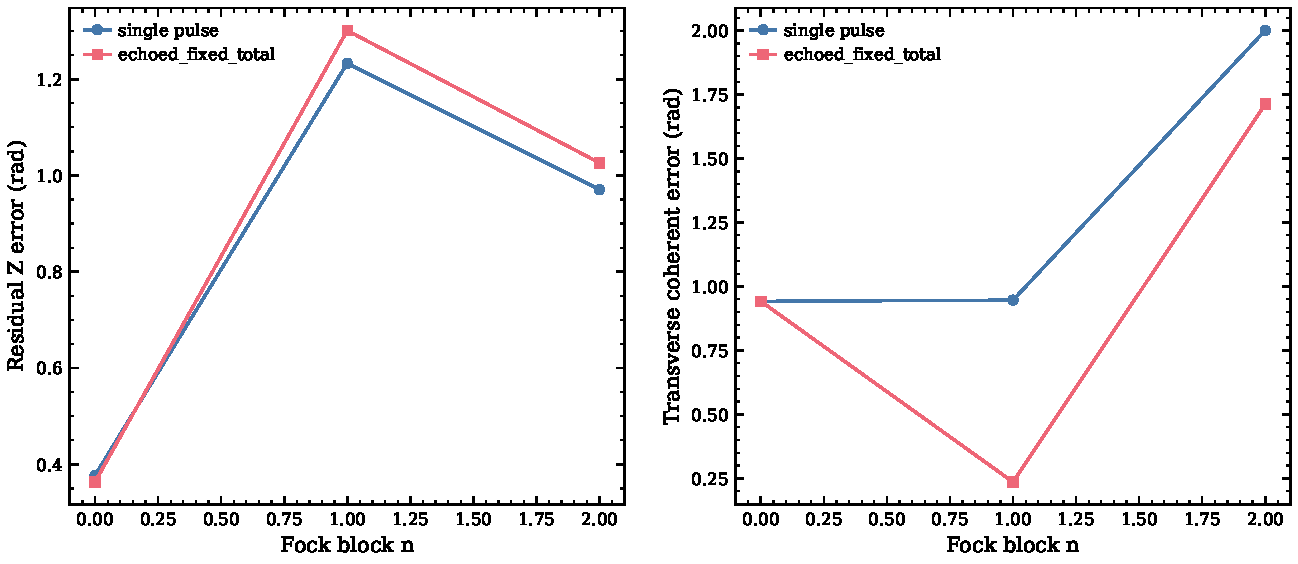
\includegraphics[width=\linewidth]{../figures/echo_block_error_breakdown.pdf}
  \caption{Residual-\(Z\) and transverse coherent-error breakdown across Fock blocks for the strongest echoed-improvement case. Echo reduces the transverse error on the middle block, but large coherent mismatch remains on the highest active block.}
  \label{fig:block-breakdown}
\end{figure}

\section{Reproducibility}

\subsection{Optimized Parameters}
Table~\ref{tab:best-single-params} records the best single-pulse tone parameters, and Table~\ref{tab:best-echo-params} records the best echoed half-SQR tone parameters. Full-precision values are stored in \texttt{artifacts/echo\_comparison/highlights/best\_single\_pulse.json} and \texttt{artifacts/echo\_comparison/highlights/best\_echoed\_sqr.json}.

\begin{table*}[t]
  \centering
  \caption{Best single-pulse parameters for \texttt{chi\_plus\_chiprime\_na2\_chiT1p0\_familyC}. Frequencies are reported as \(\omega/2\pi\).}
  \begin{tabular}{@{}cccccc@{}}
    \toprule
    Tone $n$ & $d\lambda_n$ & $d\alpha_n$ (rad) & $d\omega_n/2\pi$ (Hz) & Amplitude (Mrad/s) & Phase (rad) \\
    \midrule
    0 & -0.508596 & 0.086945 & $6.2890\times 10^{-5}$ & -1.465889 & -0.855533 \\
    1 & -0.603310 & -0.024374 & $8.5030\times 10^{-6}$ & -1.263862 & -0.464197 \\
    \bottomrule
  \end{tabular}
  \label{tab:best-single-params}
\end{table*}

\begin{table*}[t]
  \centering
  \caption{Best echoed half-SQR parameters for \texttt{chi\_only\_na3\_chiT5p0\_familyD\_seed317160} under \texttt{echoed\_fixed\_total}. The two half-SQR waveforms are identical.}
  \begin{tabular}{@{}cccccc@{}}
    \toprule
    Tone $n$ & $d\lambda_n$ & $d\alpha_n$ (rad) & $d\omega_n/2\pi$ (Hz) & Amplitude (Mrad/s) & Phase (rad) \\
    \midrule
    0 & -0.129843 & -0.008985 & $7.41\times 10^{-10}$ & 1.347042 & 1.641222 \\
    1 & -0.078647 & -0.029763 & $5.4079\times 10^{-4}$ & 0.979146 & -2.117878 \\
    2 & -0.178151 & 0.000377 & $-1.1748\times 10^{-3}$ & 0.941192 & -2.491834 \\
    \bottomrule
  \end{tabular}
  \label{tab:best-echo-params}
\end{table*}

The best echoed sequence uses the following fixed refocusing-pulse parameters:
\[
\tau_\pi = \SI{40}{ns}, \qquad \text{axis}=x, \qquad \phi_\pi = 0,
\]
with total gate duration \SI{1760.563}{ns}, active SQR duration \SI{1680.563}{ns}, and half-SQR duration \SI{840.282}{ns}.

\subsection{Waveform and Pulse Information}
The best echoed waveform samples are stored in \texttt{artifacts/echo\_comparison/waveforms/chi\_only\_na3\_chiT5p0\_familyD\_seed317160\_echoed\_fixed\_total.npz}. The corresponding JSON highlight artifact stores the full sequence specification, including the four time-ordered elements:
\begin{enumerate}
  \item half SQR, duration \SI{840.282}{ns}, start \SI{0}{ns};
  \item \(X_\pi\), duration \SI{40}{ns}, start \SI{840.282}{ns};
  \item half SQR, duration \SI{840.282}{ns}, start \SI{880.282}{ns};
  \item \(X_\pi\), duration \SI{40}{ns}, start \SI{1720.563}{ns}.
\end{enumerate}

\subsection{Gate Sequence and Decomposition}
The baseline branch is a single Gaussian multitone SQR pulse. The echoed branch is the explicit four-element sequence above with \texttt{second\_half\_transform = identical\_repeat}. The target-construction rule stored in the echoed artifact is
\[
W_n = X_\pi^\dagger \sqrt{R_n},
\]
which is the ideal repeated-half rule used to derive the half-SQR targets from the requested final block operators.

\subsection{Modeling and Simulation Assumptions}
All simulations use the closed-system dispersive model with \(K=0\), \(N_{\mathrm{tr}}=2\), and \(N_{\mathrm{cav}}=N_{\mathrm{active}}+2\) unless explicitly changed in the validation replay. The compilation step is \SI{4}{ns} in the main runs and \SI{2}{ns} in the fine-step validation replay. The echoed comparison uses the same logical basis ordering and strict active-subspace metrics as the baseline single-pulse study.

\subsection{Reproduction Procedure}
To reproduce the current report end-to-end, run the following from the study root:
\begin{enumerate}
  \item \texttt{python scripts/run\_study.py}
  \item \texttt{python scripts/validate\_results.py}
  \item \texttt{python scripts/run\_echo\_comparison.py}
  \item \texttt{python scripts/validate\_echo\_comparison.py}
  \item Open \texttt{scripts/reproducibility\_notebook.ipynb} and run the saved-output pathway.
\end{enumerate}
The expected outputs are the JSON summaries in \texttt{data/}, the figures in \texttt{figures/}, the highlight artifacts in \texttt{artifacts/echo\_comparison/highlights/}, and the validation payload \texttt{data/echo\_comparison\_validation.json}. Agreement can be checked by confirming the headline best-single and best-echoed fidelities \(0.873625\) and \(0.606132\), respectively.

\subsection{Saved Artifacts}
The most important saved artifacts are:
\begin{itemize}
  \item \texttt{artifacts/cases/chi\_plus\_chiprime\_na2\_chiT1p0\_familyC.json}: best single-pulse baseline case.
  \item \texttt{artifacts/echo\_comparison/cases/chi\_only\_na3\_chiT5p0\_familyD\_seed317160\_echoed\_fixed\_total.json}: best echoed case.
  \item \texttt{artifacts/echo\_comparison/highlights/best\_single\_pulse.json}: compact highlight artifact for the best single branch.
  \item \texttt{artifacts/echo\_comparison/highlights/best\_echoed\_sqr.json}: compact highlight artifact for the best echoed branch.
  \item \texttt{data/echo\_comparison\_summary.json}: branch means, family summaries, and matched-delta tables.
  \item \texttt{data/echo\_comparison\_validation.json}: extension-specific validation checks.
\end{itemize}
These files are sufficient to reload the optimized parameters, the restricted operators, the sequence specification, the waveform samples, and the validation verdict without rerunning the optimization.

\end{document}